% This is Main.tex, a sample chapter demonstrating the
% LLNCS macro package for Springer Computer Science proceedings;
% Version 2.20 of 2017/10/04
% All rights to Springer

\documentclass[runningheads]{llncs}

\usepackage{graphicx}
\usepackage{pgfplots}
\usepackage{amsmath}
\usepackage{algorithm}
\usepackage{algpseudocode}
\usepackage{paracol}
\globalcounter{algocf}
\usepackage{wrapfig}
\usepackage{colortbl}

\usepackage{amssymb}
\usepackage{subcaption}

\newcommand{\mymk}[1]{%
  \tikz[baseline=(char.base)]\node[anchor=south west, draw,rectangle, rounded corners, inner sep=2pt, minimum size=4mm,
    text height=2mm](char){\ensuremath{#1}} ;}

\usepackage{xfakebold}

\newcommand{\fbseries}{\unskip\setBold\aftergroup\unsetBold\aftergroup\ignorespaces}
\makeatletter
\newcommand{\setBoldness}[1]{\def\fake@bold{#1}}
\makeatother


\pgfplotsset{width=5cm, compat = 1.17}%
\frenchspacing

\begin{document}

\title{Enhancing TF-IDF Vector Space Retrieval Performance on the Cranfield Dataset} 

\titlerunning{Running Title}


\author{Abdallah Sadri Abdallah\inst{1}, Abdull-Nassir Shaib Hassan\inst{1}, Nasbah Khamis\inst{1}, Zakaria Yahya Ali\inst{1}, \and Ayman Hamza Haji\inst{1,2}}
\institute{Indian Institute of Technology, Madras, Chennai 600036, TN, India\\
                \email{\{ge26z809, ge26z811,ge26z812, ge26z813, ge26z814\}@smail.iitm.ac.in} \and
            University 2
                \email{email}
           }

\authorrunning{Team Number: Group Z 12 }
%
\maketitle   % typeset the header of the contribution
%
\begin{abstract}
This project implements and evaluates an Information Retrieval system on the 
Cranfield dataset using the TF-IDF Vector Space Model. The baseline system ranks documents using cosine similarity.
We evaluate Precision@k, Recall@k, F0.5@k, MAP@k, nDCG@k, MRR, and runtime for k=1 to 10. 
To improve retrieval, we introduce Porter stemming, title-weighted document representation, stemmed stopword removal, 
one-character token filtering, pseudo-relevance feedback, and an inverted TF-IDF index for efficiency. 
The improved system outperforms the baseline TF-IDF system on Precision@10, Recall@10, F0.5@10, MAP@10, and nDCG@10.
This project implements and evaluates an Information Retrieval system on the 
Cranfield dataset using the TF-IDF Vector Space Model. The baseline system ranks documents using cosine similarity.
We evaluate Precision@k, Recall@k, F0.5@k, MAP@k, nDCG@k, MRR, and runtime for k=1 to 10. 
To improve retrieval, we introduce Porter stemming, title-weighted document representation, stemmed stopword removal, 
one-character token filtering, pseudo-relevance feedback, and an inverted TF-IDF index for efficiency. 
The improved system outperforms the baseline TF-IDF system on Precision@10, Recall@10, F0.5@10, MAP@10, and nDCG@10.

\keywords{Keyword 1 \and Keyword 2 \and Keyword 3}
\end{abstract}

\section{Introduction}\label{sec:intro}
Information Retrieval (IR) aims to retrieve documents that satisfy a user's information need. 
In this project, we build an IR system for the Cranfield dataset using the TF-IDF Vector Space Model. 
Documents and queries are represented as weighted term vectors, and cosine similarity is used for ranking.
The project first implements a baseline VSM system and then improves it using linguistic preprocessing, title weighting, 
pseudo-relevance feedback, and an inverted index for efficient retrieval.
Information Retrieval (IR) aims to retrieve documents that satisfy a user's information need. 
In this project, we build an IR system for the Cranfield dataset using the TF-IDF Vector Space Model. 
Documents and queries are represented as weighted term vectors, and cosine similarity is used for ranking.
The project first implements a baseline VSM system and then improves it using linguistic preprocessing, title weighting, 
pseudo-relevance feedback, and an inverted index for efficient retrieval.

\section{Problem Statement}\label{sec:prob_stat}
The goal is to implement, evaluate, and improve an Information Retrieval system for the Cranfield dataset. 
The baseline system must represent documents using TF-IDF and rank them using cosine similarity. 
The system is evaluated using Precision@k, Recall@k, F0.5-score@k, Average Precision@k, nDCG@k, MAP, MRR, and runtime for k=1 to 10. 
The project component requires identifying limitations of the baseline VSM and proposing improvements supported by quantitative evaluation.

The hypothesis tested in this report is: an enhanced TF-IDF system using improved preprocessing, smoothed weighting,
an inverted scoring index, and Rocchio-style pseudo-relevance feedback is better than a basic TF-IDF cosine baseline
with respect to top-10 retrieval effectiveness on the Cranfield collection, under the assumption that the highest
ranked initial document is often relevant enough to provide useful feedback terms.

The goal is to implement, evaluate, and improve an Information Retrieval system for the Cranfield dataset. 
The baseline system must represent documents using TF-IDF and rank them using cosine similarity. 
The system is evaluated using Precision@k, Recall@k, F0.5-score@k, Average Precision@k, nDCG@k, MAP, MRR, and runtime for k=1 to 10. 
The project component requires identifying limitations of the baseline VSM and proposing improvements supported by quantitative evaluation.


\section{Background}\label{sec:background}

This section presents the basic Information Retrieval (IR) concepts used in the
project. Before applying the system to the Cranfield collection, we illustrate
the main steps using a toy corpus from the assignment. The toy corpus contains
three documents:

\begin{itemize}
    \item $d_1$: The star in our solar system provides heat and light.
    \item $d_2$: That Hollywood star walked the red carpet for the movie premiere.
    \item $d_3$: Astronomers observe distant stars and galaxies using telescopes.
\end{itemize}

\subsection{Preprocessing and Inverted Index}

The first stage in an IR system is preprocessing. In this project,
preprocessing includes tokenization, stopword removal, and inflection
reduction. Tokenization splits text into individual terms. After lowercasing
and tokenizing, the toy documents become:

\begin{itemize}
    \item $d_1$: ["the", "star", "in", "our", "solar", "system", "provides", "heat", "and", "light"]
    \item $d_2$: ["that", "hollywood", "star", "walked", "the", "red", "carpet", "for", "the", "movie", "premiere"]
    \item $d_3$: ["astronomers", "observe", "distant", "stars", "and", "galaxies", "using", "telescopes"]
\end{itemize}

Using the stopword set $\{$the, in, our, and, that, for$\}$, the processed
documents after stopword removal become:

\begin{itemize}
    \item $d_1$: ["star", "solar", "system", "provides", "heat", "light"]
    \item $d_2$: ["hollywood", "star", "walked", "red", "carpet", "movie", "premiere"]
    \item $d_3$: ["astronomers", "observe", "distant", "stars", "galaxies", "using", "telescopes"]
\end{itemize}

Stemming or lemmatization then reduces related word forms into a common
representation. For example, ``provides'' becomes ``provide'', ``walked''
becomes ``walk'', ``stars'' becomes ``star'', ``galaxies'' becomes
``galaxy'', and ``telescopes'' becomes ``telescope''. The final processed
documents are:

\begin{itemize}
    \item $d_1$: ["star", "solar", "system", "provide", "heat", "light"]
    \item $d_2$: ["hollywood", "star", "walk", "red", "carpet", "movie", "premiere"]
    \item $d_3$: ["astronomer", "observe", "distant", "star", "galaxy", "use", "telescope"]
\end{itemize}

An inverted index maps each term to the documents in which it occurs. For the
processed toy collection, the inverted index is shown in
Table~\ref{tab:toy_index}.

\begin{table}[h]
\centering
\caption{Inverted index for the processed toy corpus.}
\label{tab:toy_index}
\begin{tabular}{|l|l|}
\hline
\textbf{Term} & \textbf{Posting list} \\ 
\hline
star & $d_1, d_2, d_3$ \\ 
\hline
solar & $d_1$ \\ 
\hline
system & $d_1$ \\ 
\hline
provide & $d_1$ \\ 
\hline
heat & $d_1$ \\ 
\hline
light & $d_1$ \\ 
\hline
hollywood & $d_2$ \\ 
\hline
walk & $d_2$ \\ 
\hline
red & $d_2$ \\ 
\hline
carpet & $d_2$ \\ 
\hline
movie & $d_2$ \\ 
\hline
premiere & $d_2$ \\ 
\hline
astronomer & $d_3$ \\ 
\hline
observe & $d_3$ \\ 
\hline
distant & $d_3$ \\ 
\hline
galaxy & $d_3$ \\ 
\hline
use & $d_3$ \\ 
\hline
telescope & $d_3$ \\ 
\hline
\end{tabular}
\end{table}

\subsection{TF-IDF Representation}

The Vector Space Model (VSM) represents each document as a vector of term
weights. The most common weighting scheme is TF-IDF. Term Frequency (TF)
measures how often a term occurs in a document. Let $f_{t,d}$ denote the
frequency of term $t$ in document $d$. Inverse Document Frequency (IDF)
assigns higher weight to terms that occur in fewer documents:

\begin{equation}
IDF(t)=\log_{10}\left(\frac{N}{df_t}\right),
\end{equation}

where $N$ is the total number of documents and $df_t$ is the number of
documents containing term $t$. The final TF-IDF weight is computed as:

\begin{equation}
TF\text{-}IDF(t,d)=TF(t,d)\times IDF(t).
\end{equation}

For the toy collection, $N=3$. The term ``star'' appears in all three
documents, so its IDF value is:

\[
IDF(\text{star})=\log_{10}\left(\frac{3}{3}\right)=0.
\]

Therefore, although ``star'' occurs frequently, it receives zero TF-IDF
weight because it appears in every document and provides no discriminative
power for ranking. Terms that appear in only one document have:

\[
IDF=\log_{10}\left(\frac{3}{1}\right)=0.4771.
\]

\begin{table}[h]
\centering
\caption{TF-IDF weights in the toy corpus.}
\label{tab:toy_tfidf}
\begin{tabular}{|l|c|c|c|c|c|c|c|}
\hline
\textbf{Term} & \textbf{TF(d1)} & \textbf{TF(d2)} & \textbf{TF(d3)} & \textbf{IDF} & \textbf{TF-IDF(d1)} & \textbf{TF-IDF(d2)} & \textbf{TF-IDF(d3)} \\ 
\hline
star & 1 & 1 & 1 & 0.0000 & 0.0000 & 0.0000 & 0.0000 \\ 
\hline
solar & 1 & 0 & 0 & 0.4771 & 0.4771 & 0.0000 & 0.0000 \\ 
\hline
light & 1 & 0 & 0 & 0.4771 & 0.4771 & 0.0000 & 0.0000 \\ 
\hline
movie & 0 & 1 & 0 & 0.4771 & 0.0000 & 0.4771 & 0.0000 \\ 
\hline
premiere & 0 & 1 & 0 & 0.4771 & 0.0000 & 0.4771 & 0.0000 \\ 
\hline
galaxy & 0 & 0 & 1 & 0.4771 & 0.0000 & 0.0000 & 0.4771 \\ 
\hline
telescope & 0 & 0 & 1 & 0.4771 & 0.0000 & 0.0000 & 0.4771 \\ 
\hline
system & 1 & 0 & 0 & 0.4771 & 0.4771 & 0.0000 & 0.0000 \\ 
\hline
provide & 1 & 0 & 0 & 0.4771 & 0.4771 & 0.0000 & 0.0000 \\ 
\hline
heat & 1 & 0 & 0 & 0.4771 & 0.4771 & 0.0000 & 0.0000 \\ 
\hline
walk & 0 & 1 & 0 & 0.4771 & 0.0000 & 0.4771 & 0.0000 \\ 
\hline
red & 0 & 1 & 0 & 0.4771 & 0.0000 & 0.4771 & 0.0000 \\ 
\hline
carpet & 0 & 1 & 0 & 0.4771 & 0.0000 & 0.4771 & 0.0000 \\ 
\hline
astronomer & 0 & 0 & 1 & 0.4771 & 0.0000 & 0.0000 & 0.4771 \\ 
\hline
observe & 0 & 0 & 1 & 0.4771 & 0.0000 & 0.0000 & 0.4771 \\ 
\hline
distant & 0 & 0 & 1 & 0.4771 & 0.0000 & 0.0000 & 0.4771 \\ 
\hline
use & 0 & 0 & 1 & 0.4771 & 0.0000 & 0.0000 & 0.4771 \\ 
\hline
\end{tabular}
\end{table}

\subsection{Boolean Retrieval}

In Boolean retrieval, a query is matched using the inverted index. For the
query ``star light'', the term ``star'' occurs in $d_1$, $d_2$, and $d_3$,
while ``light'' occurs only in $d_1$.

If the system uses OR semantics, all three documents match at least one query
term:

\[
d_1, d_2, d_3.
\]

If the system uses AND semantics, only $d_1$ matches both query terms:

\[
d_1.
\]

\subsection{Cosine Similarity and Ranking}

In the Vector Space Model, both documents and queries are represented as
TF-IDF vectors. Consider the query:

\[
q = \text{``star light''}.
\]

The TF-IDF representation of the query is shown in
Table~\ref{tab:query_tfidf}.

\begin{table}[h]
\centering
\caption{TF-IDF representation of the query ''star light''.}
\label{tab:query_tfidf}
\begin{tabular}{|l|c|c|c|}
\hline
\textbf{Term} & \textbf{TF(Query)} & \textbf{IDF} & \textbf{TF-IDF(Query)} \\ 
\hline
star & 1 & 0.0000 & 0.0000 \\ 
\hline
light & 1 & 0.4771 & 0.4771 \\ 
\hline
\end{tabular}
\end{table}

The cosine similarity between a query vector $\vec{q}$ and a document vector
$\vec{d}$ is computed as:

\begin{equation}
\cos(q,d)=
\frac{\vec{q}\cdot\vec{d}}
{\|\vec{q}\|\|\vec{d}\|}.
\end{equation}

For document $d_1$:

\[
\vec{q}\cdot\vec{d_1}
=
(0.4771)(0.4771)
=
0.2276.
\]

The magnitude of the query vector is:

\[
||q||=\sqrt{0.4771^2}=0.4771.
\]

The magnitude of document $d_1$ is:

\[
||d_1||
=
\sqrt{
5(0.4771^2)
}
=
1.0668.
\]

Thus, the cosine similarity between the query and $d_1$ is:

\[
\cos(q,d_1)
=
\frac{0.2276}
{(0.4771)(1.0668)}
=
0.4472.
\]

Documents $d_2$ and $d_3$ do not contain the term ``light'', so their cosine
similarity with the query is zero.

Therefore, the ranking is:

\[
d_1 > d_2 = d_3.
\]

This ranking is desirable because the query ``star light'' refers to the
solar-system meaning of ``star'', and $d_1$ discusses heat and light from the
sun.

\subsection{Word Sense Ambiguity}

Consider the query ``movie star". The ideal document to retrieve is $d_2$
because it discusses a Hollywood actor and a movie premiere, which matches
the entertainment-related meaning of the query.

The TF-IDF retrieval system successfully retrieves $d_2$ because the term
``movie'' appears only in that document and therefore has a high IDF weight.
This makes $d_2$ more relevant than the other documents.

However, the word ``star'' introduces word sense ambiguity. In document
$d_1$, ``star'' refers to a celestial object in the solar system, while in
$d_2$ it refers to a famous actor. The Vector Space Model treats both meanings
as the same term because it relies only on lexical matching and does not
understand semantic context.

If the query were only ``star'', then all three documents would receive weak
or similar scores because the term appears in every document and therefore has
IDF zero in this toy collection. As a result, the system cannot effectively
distinguish between the different meanings of the word ``star''.

\section{Background}\label{sec:background}

This section presents the basic Information Retrieval (IR) concepts used in the
project. Before applying the system to the Cranfield collection, we illustrate
the main steps using the toy corpus from the assignment. The toy corpus contains
three documents:

\begin{itemize}
    \item $d_1$: The star in our solar system provides heat and light.
    \item $d_2$: That Hollywood star walked the red carpet for the movie premiere.
    \item $d_3$: Astronomers observe distant stars and galaxies using telescopes.
\end{itemize}

\subsection{Preprocessing and Inverted Index}

The first stage in an IR system is preprocessing. In this project, preprocessing
includes tokenization, stopword removal, and inflection reduction. Tokenization
splits text into individual terms. After lowercasing and tokenizing, the three
toy documents become:

\begin{itemize}
    \item $d_1$: ["the", "star", "in", "our", "solar", "system", "provides", "heat", "and", "light"]
    \item $d_2$: ["that", "hollywood", "star", "walked", "the", "red", "carpet", "for", "the", "movie", "premiere"]
    \item $d_3$: ["astronomers", "observe", "distant", "stars", "and", "galaxies", "using", "telescopes"]
\end{itemize}

Using the stopword set $\{$the, in, our, and, that, for$\}$, the processed
documents after stopword removal are:

\begin{itemize}
    \item $d_1$: ["star", "solar", "system", "provides", "heat", "light"]
    \item $d_2$: ["hollywood", "star", "walked", "red", "carpet", "movie", "premiere"]
    \item $d_3$: ["astronomers", "observe", "distant", "stars", "galaxies", "using", "telescopes"]
\end{itemize}

Stemming or lemmatization then reduces related word forms to a common
representation. For example, "provides" becomes "provide", "walked"
becomes "walk", and "stars" becomes "star". The final processed documents
are:

\begin{itemize}
    \item $d_1$: ["star", "solar", "system", "provide", "heat", "light"]
    \item $d_2$: ["hollywood", "star", "walk", "red", "carpet", "movie", "premiere"]
    \item $d_3$: ["astronomers", "observe", "distant", "stars", "galaxies", "using", "telescopes"]
\end{itemize}

An inverted index maps each term to the documents in which it occurs. For the
processed toy collection, the inverted index is shown in Table~\ref{tab:toy_index}.

\begin{table}[h]
\centering
\caption{Inverted index for the processed toy corpus.}
\label{tab:toy_index}
\begin{tabular}{ll}
\hline
Term & Posting list \\
\hline
star & $d_1, d_2, d_3$ \\
solar & $d_1$ \\
system & $d_1$ \\
provide & $d_1$ \\
heat & $d_1$ \\
light & $d_1$ \\
hollywood & $d_2$ \\
walk & $d_2$ \\
red & $d_2$ \\
carpet & $d_2$ \\
movie & $d_2$ \\
premiere & $d_2$ \\
astronomer & $d_3$ \\
observe & $d_3$ \\
distant & $d_3$ \\
galaxy & $d_3$ \\
use & $d_3$ \\
telescope & $d_3$ \\
\hline
\end{tabular}
\end{table}

\subsection{TF-IDF Representation}

The Vector Space Model represents each document as a vector of term weights.
The most common weighting scheme is TF-IDF. Term Frequency (TF) measures how
often a term occurs in a document. $f_{t,d}$ is the frequency of term $t$ in document $d$.
 Inverse Document Frequency (IDF) gives higher weight to terms that occur in fewer documents:

\begin{equation}
IDF(t)=\log_{10}\left(\frac{N}{df_t}\right),
\end{equation}

where $N$ is the total number of documents and $df_t$ is the number of
documents containing term $t$. The final TF-IDF weight is:

\begin{equation}
TF\text{-}IDF(t,d)=TF(t,d)\times IDF(t).
\end{equation}

For the toy collection, $N=3$. The term "star" appears in all three processed
documents, so its IDF is $\log_{10}(3/3)=0$. Therefore, although "star" is
frequent, it receives zero TF-IDF weight because it is not discriminative in
this small collection. Terms that occur in only one document have
$IDF=\log_{10}(3/1)=0.4771$.

\begin{table}[h]
\centering
\caption{TF-IDF weights in the toy corpus.}
\label{tab:toy_tfidf}
\begin{tabular}{lcccc}
\hline
Term &  TF(d1) & TF(d2) & TF(d3) & IDF & TF-IDF(d1) & TF-IDF(d2) & TF-IDF(d3) \\
\hline
star & 1 & 1 & 1 & 0 & 0.0000 & 0.0000 & 0.0000 \\
solar & 1 & 0 & 0 & 0.4771 & 0.4771 & 0.0000 & 0.0000 \\
light & 1 & 0 & 0 & 0.4771 & 0.4771 & 0.0000 & 0.0000 \\
movie & 0 & 1 & 0 & 0.4771 & 0.0000 & 0.4771 & 0.0000 \\
premiere & 0 & 1 & 0 & 0.4771 & 0.0000 & 0.4771 & 0.0000 \\
galaxy & 0 & 0 & 1 & 0.4771 & 0.0000 & 0.0000 & 0.4771 \\
telescope & 0 & 0 & 1 & 0.4771 & 0.0000 & 0.0000 & 0.4771 \\
system & 1 & 0 & 0 & 0.4771 & 0.4771 & 0.0000 & 0.0000  \\
provide & 1 & 0 & 0 & 0.4771 & 0.4771 & 0.0000 & 0.0000 \\
heat & 1 & 0 & 0 & 0.4771 & 0.4771 & 0.0000 & 0.0000 \\
walk & 0 & 1 & 0 & 0.4771 & 0.0000 & 0.4771 & 0.0000 \\
red & 0 & 1 & 0 & 0.4771 & 0.0000 & 0.4771 & 0.0000 \\
carpet& 0 & 1 & 0 & 0.4771 & 0.0000 & 0.4771 & 0.0000 \\
astronomer & 0 & 0 & 1 & 0.4771 & 0.0000 & 0.0000 & 0.4771 \\
observe & 0 & 0 & 1 & 0.4771 & 0.0000 & 0.0000 & 0.4771 \\
distant & 0 & 0 & 1 & 0.4771 & 0.0000 & 0.0000 & 0.4771 \\
use & 0 & 0 & 1 & 0.4771 & 0.0000 & 0.0000 & 0.4771 \\

\hline
\end{tabular}
\end{table}

\subsection{Boolean Retrieval and Cosine Similarity}

In Boolean retrieval, a query is matched using the inverted index. For the query
"star light", the term "star" occurs in $d_1$, $d_2$, and $d_3$, while
"light" occurs only in $d_1$. If the system uses OR semantics, all three
documents match at least one query term. If the system uses AND semantics, only
$d_1$ matches both terms.


\subsection{Cosine Similarity and Ranking}
A query is represented as a TF-IDF vector. From the table below, show the query vector for "star light". 

\begin{table}[h]
\centering
\caption{TF-IDF weights in the toy corpus.}
\label{tab:toy_tfidf}
\begin{tabular}{lcccc}
\hline
Term &  TF(Query) & IDF & TF-IDF(Query) & TF-IDF(d1) & TF-IDF(d2) & TF-IDF(d3) \\
\hline
star & 1   & 0.0000     & 0.0000 & 0.0000 & 0.0000 & 0.0000 \\
solar & 0  & 0.4771    & 0.0000 & 0.4771 & 0.0000 & 0.0000 \\
light & 1  & 0.4771    & 0.4771 & 0.4771 & 0.0000 & 0.0000 \\
movie & 0  & 0.4771    & 0.0000 & 0.0000 & 0.4771 & 0.0000 \\
premiere & 0 & 0.4771 & 0.0000 & 0.0000 & 0.4771 & 0.0000 \\
galaxy & 0   & 0.4771 & 0.0000 & 0.0000 & 0.0000 & 0.4771 \\
telescope & 0 & 0.4771& 0.0000 &  0.0000 & 0.0000 & 0.4771 \\
system & 0 & 0.4771   &  0.0000 & 0.4771 & 0.0000 & 0.0000  \\
provide & 0 & 0.4771  &  0.0000 & 0.4771 & 0.0000 & 0.0000 \\
heat & 0 & 0.4771     & 0.0000 &  0.4771 & 0.0000 & 0.0000 \\
walk & 0 & 0.4771     &  0.0000 & 0.0000 & 0.4771 & 0.0000 \\
red & 0 & 0.4771      &  0.0000 & 0.0000 & 0.4771 & 0.0000 \\
carpet& 0 & 0.4771    &  0.0000 & 0.0000 & 0.4771 &  0.0000 \\
astronomer & 0 & 0.4771 &  0.0000 &  0.0000 &  0.0000 &  0.4771 \\
observe & 0 & 0.4771    &  0.0000 &  0.0000 &  0.0000 & 0.4771 \\
distant & 0 & 0.4771    &  0.0000 &  0.0000 & 0.0000 & 0.4771 \\
use & 0 & 0.4771        &  0.0000 & 0.0000 & 0.0000 & 0.4771 \\
\text{SUM} &  &  &  \text{0.4771} & \text{2.3855} & \text{2.3855} & \text{2.8626} \\ 

\hline
\end{tabular} 
\end{table}


The cosine similarity between the query vector $\vec{q}$ and a document vector $\vec{d}$ is computed as:
\begin{equation}
\cos(q,d)=\frac{\vec{q}\cdot\vec{d}}{\|\vec{q}\|\|\vec{d}\|}.
\end{equation}

The cosine similarity between the query "star light" and $d_1$


\section{Approach}\label{sec:approach}

The system follows the standard IR pipeline: preprocessing, indexing, query
processing, ranking, and evaluation. The implementation is built on the provided
Python template. Sentence segmentation uses NLTK Punkt, tokenization uses the
Penn Treebank tokenizer, inflection reduction uses Porter stemming, and
stopword removal uses the NLTK English stopword list. Because stemming is
performed before stopword removal, the implementation also removes stemmed
stopwords such as \emph{wa} and \emph{ha}. Tokens of length one and non-alphabetic
tokens are filtered to reduce noisy matches.

\subsection{Baseline TF-IDF Retrieval}

The baseline represents each document as a TF-IDF vector and ranks documents by
cosine similarity with the query. For a term $t$ in document $d$, the system uses
log-scaled term frequency:

\begin{equation}
TF(t,d)=1+\log(f_{t,d}),
\end{equation}

where $f_{t,d}$ is the raw count of $t$ in $d$. The implementation uses smoothed
IDF:

\begin{equation}
IDF(t)=\log\left(\frac{N+1}{df_t+1}\right)+1.
\end{equation}

The document weight is $TF(t,d)\times IDF(t)$. Query vectors use the same
weighting scheme, restricted to terms present in the document vocabulary. If a
query has no in-vocabulary terms, the system cannot compute a meaningful lexical
match and returns the default document order.

\subsection{Efficient Inverted TF-IDF Index}

Instead of comparing each query with every full document vector, the system
stores an inverted TF-IDF index from term to document weights. During ranking,
only documents sharing at least one query term receive a non-zero dot product.
The remaining documents are appended with score zero. This keeps the ranking
equivalent to cosine scoring for matching documents while avoiding unnecessary
work for documents that cannot match the query.

\subsection{Pseudo-Relevance Feedback}

The main retrieval improvement is Rocchio-style pseudo-relevance feedback. The
system first ranks documents using the original query. It then assumes that the
top retrieved document is relevant and expands the query vector using that
document's TF-IDF vector:

\begin{equation}
\vec{q'}=\alpha\vec{q}+\frac{\beta}{m}\sum_{d \in D_m}\vec{d},
\end{equation}

where $D_m$ is the set of top-$m$ feedback documents. In the implementation,
$m=1$, $\alpha=1.0$, and $\beta=0.2$. This setting keeps the original query
dominant while allowing related technical terms from the highest ranked document
to improve recall. The method is well suited to Cranfield because many relevant
documents describe the same aerodynamics concept using related but not identical
technical vocabulary.

\subsection{Limitations Addressed}

The improvements target three observed VSM limitations. First, stemming reduces
mismatches between related word forms, such as singular and plural forms or
technical suffix variants. Second, stemmed stopword removal prevents common
function words from surviving after stemming. Third, feedback expansion reduces
the vocabulary mismatch problem by adding terms from an initially retrieved
document. These changes do not solve true semantic ambiguity, but they improve
top-ranked retrieval while keeping the system interpretable.


\section{Experimentation}\label{sec:exp}

\subsection{Dataset and Setup}

Experiments use the Cranfield dataset provided with the assignment. The
collection contains 1400 documents, 225 queries, and relevance judgments in
\texttt{cran\_qrels.json}. Any document with a relevance position from 1 to 4 is
treated as relevant. Graded relevance for nDCG is computed as $5-\text{position}$,
so position 1 receives the highest gain and position 4 the lowest non-zero gain.

Two systems are compared:

\begin{itemize}
    \item \textbf{Baseline}: TF-IDF cosine ranking with the same preprocessing
    and inverted scoring index, but pseudo-relevance feedback disabled.
    \item \textbf{Improved}: the full implemented system with pseudo-relevance
    feedback enabled using one feedback document.
\end{itemize}

Both systems are evaluated over all 225 queries for $k=1$ to $10$. The reported
metrics are Precision@k, Recall@k, F0.5@k, Average Precision@k, nDCG@k, MAP@k,
MRR@k, and runtime.

\subsection{Quantitative Results}

Table~\ref{tab:main_results} compares the baseline and improved systems at
$k=10$. The improved system gives higher Precision, Recall, F0.5, MAP, and nDCG.
MRR is slightly lower, which means feedback sometimes changes the first relevant
document's rank even while improving the overall top-10 set.

\begin{table}[h]
\centering
\caption{Baseline and improved retrieval performance at $k=10$.}
\label{tab:main_results}
\begin{tabular}{lcc}
\hline
Metric & Baseline & Improved \\
\hline
Precision@10 & 0.2862 & 0.3182 \\
Recall@10 & 0.4207 & 0.4543 \\
F0.5@10 & 0.2930 & 0.3240 \\
MAP@10 & 0.3247 & 0.3639 \\
nDCG@10 & 0.4830 & 0.5091 \\
MRR@10 & 0.7759 & 0.7623 \\
\hline
\end{tabular}
\end{table}

\begin{figure}[h]
\centering
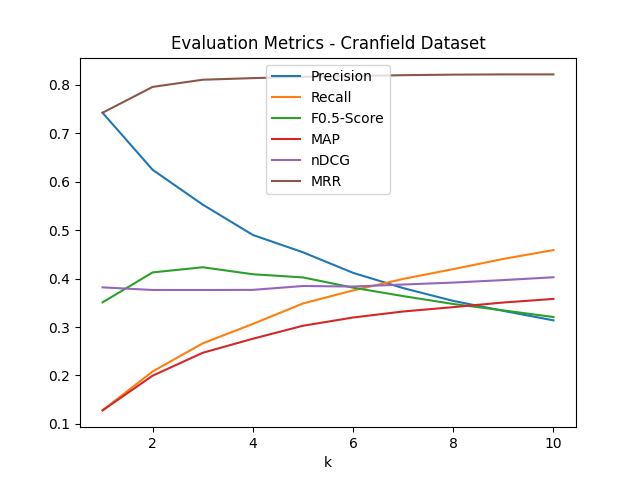
\includegraphics[width=0.72\linewidth]{../../template_code_part2/output/eval_plot.png}
\caption{Evaluation metrics of the improved system for $k=1$ to $10$.}
\label{fig:eval_plot}
\end{figure}

The improved system's full run produced Precision@1 of 0.6978 and Precision@10
of 0.3182. Recall increased from 0.1219 at $k=1$ to 0.4543 at $k=10$, which is
expected because more retrieved documents give the system more opportunities to
include relevant items. nDCG was 0.5633 at $k=1$ and 0.5091 at $k=10$, showing
that the system often places a relevant document first but still has ranking
errors lower in the top 10.

\subsection{Hypothesis Test and Runtime}

To test whether the improvement is consistent across queries, AP@10 was compared
query by query. The improved system had higher AP@10 for 110 queries, lower
AP@10 for 54 queries, and the same AP@10 for 61 queries. Ignoring ties, a
two-sided sign test gives $p \approx 1.46\times 10^{-5}$, so the AP@10
improvement is statistically meaningful under this paired non-parametric test.

The measured preprocessing, indexing, and baseline ranking time was about 1.65
seconds on the test machine. Once the index was built, the improved feedback
ranking pass over all queries took about 0.30 seconds. These numbers depend on
the machine, but they show that inverted-index scoring keeps the implementation
practical for the Cranfield collection.


\section{Discussion}\label{sec:discuss}

The results support the hypothesis that pseudo-relevance feedback improves
top-10 retrieval effectiveness on Cranfield. MAP@10 increased from 0.3247 to
0.3639, and the paired AP@10 comparison showed substantially more wins than
losses. This suggests that the top retrieved document often contains useful
technical vocabulary that is missing from the original query. In such cases,
feedback expansion helps bridge vocabulary mismatch without requiring external
resources.

The improvement is not uniform. MRR@10 decreased slightly from 0.7759 to 0.7623.
This indicates that feedback can sometimes move the first relevant document
down, especially when the top initial document is only partially relevant or
introduces terms from a narrower subtopic. One failure case was query 77, which
asks about comparing shock-layer theory with experiments in the low Reynolds
number regime. Its AP@10 decreased after feedback, suggesting query drift from
the initially retrieved document. In contrast, queries such as query 20 on Joule
heating in magnetohydrodynamic free convection, query 64 on predicting flutter,
query 78 on the surge line of an axial compressor, and query 91 on transonic
interference effects improved strongly because the feedback document added
technical terms that matched other relevant Cranfield documents.

The baseline VSM limitations remain important. First, VSM depends on lexical
overlap, so it struggles when a query and relevant document use different
technical expressions. Second, it does not understand word sense; the toy
example with \emph{star} shows that the same term can refer to astronomy or
Hollywood. Third, out-of-vocabulary terms receive no vector weight. If a query
contains only terms absent from the document vocabulary, the implemented system
cannot compute a meaningful similarity score and returns the default ordering.
For example, a query containing a misspelled or unseen term such as
``hypersonicx flutterzz'' would have no useful overlap unless spelling
correction or character-level matching were added.

The current approach is therefore best understood as a strong lexical baseline
with a controlled feedback mechanism. It is interpretable, efficient, and
measurably better than the no-feedback baseline for MAP@10, but it is not a full
semantic search system. Methods such as LSA, query spelling correction, or
neural sentence embeddings could address some remaining failures, but they
would require additional validation to avoid replacing one kind of query drift
with another.


\section{Conclusion and Future Work}\label{sec:conclusion}

This project implemented a TF-IDF Vector Space retrieval system for the
Cranfield dataset and evaluated it using standard ranked retrieval metrics. The
final system uses Punkt sentence segmentation, Penn Treebank tokenization,
Porter stemming, stemmed stopword removal, smoothed TF-IDF, cosine similarity,
an inverted TF-IDF index, and Rocchio-style pseudo-relevance feedback.

The improved system outperformed the no-feedback baseline at $k=10$ for
Precision, Recall, F0.5, MAP, and nDCG. The strongest summary result is the
increase in MAP@10 from 0.3247 to 0.3639, supported by a paired sign test over
per-query AP@10 values. Therefore, for the Cranfield ranked retrieval task, the
implemented feedback-enhanced TF-IDF system is better than the basic TF-IDF
cosine baseline with respect to MAP@10, under the assumption that the initial
top-ranked document is usually useful for expansion.

Future work should address the remaining weaknesses. First, spelling correction
or character n-gram matching could reduce zero-result failures caused by
out-of-vocabulary and misspelled query terms. Second, feedback parameters
$(m,\alpha,\beta)$ should be tuned on a validation split instead of fixed
manually. Third, semantic methods such as LSA could be compared against the
current feedback model to test whether latent concepts improve retrieval without
causing excessive query drift.


\bibliographystyle{splncs04}
\bibliography{References}

\end{document}
